%=============================================================================%
% Author: 	John Joseph Valletta
% Date: 	30/05/2017
% Title: 	Python workshop: Advanced topics
%=============================================================================%

%=============================================================================%
% Preamble
%=============================================================================%
% Libraries
\documentclass[pdf]{beamer}
\usepackage[export]{adjustbox}
\usepackage{framed}
\usepackage{color}
\definecolor{dkgreen}{rgb}{0,0.6,0}
\definecolor{gray}{rgb}{0.5,0.5,0.5}
\definecolor{mauve}{rgb}{0.58,0,0.82}
\definecolor{deepblue}{rgb}{0,0,0.5}
\definecolor{deepred}{rgb}{0.6,0,0}
\definecolor{deepgreen}{rgb}{0,0.5,0}
\definecolor{lightgray}{rgb}{0.92,0.92,0.92}
\usepackage{listings} % to insert code
\usepackage{textpos} % textblock
\usepackage{dirtree} % to make directory trees
\usepackage{hyperref}
\hypersetup{colorlinks=true, urlcolor=blue, linkcolor=black} 

% Listing set up
% Python
\lstdefinestyle{python}{
language=python,
formfeed=\newpage,
basicstyle=\scriptsize\ttfamily,
commentstyle=\color{deepgreen},%\color{gray},
%numbers=left,
%numberstyle=\tiny\color{gray},
stepnumber=1,
numbersep=5pt,
backgroundcolor=\color{lightgray},%\color{white},
showspaces=false,
showstringspaces=false,
showtabs=false,
frame=lines,
tabsize=4,
captionpos=b,
breaklines=true,
breakatwhitespace=false,
title=\lstname,
escapeinside={},
keywordstyle=\color{deepblue},
emphstyle=\color{deepred},
stringstyle=\color{mauve},
morekeywords={as, lambda}
}

% Presentation configuration
\mode<presentation>{\usetheme{Madrid}}
\definecolor{tealblue}{rgb}{0, 0.5, 0.5}
\usecolortheme[named=tealblue]{structure}
\useinnertheme{circles} % circles, rectanges, rounded, inmargin
\usefonttheme[onlymath]{serif} % makes math fonts like the usual LaTeX ones
\setbeamercovered{transparent=4} % transparent
\setbeamertemplate{caption}{\raggedright\insertcaption\par} % Remove the word "Figure" from caption %\setbeamertemplate{caption}[default]
\setbeamertemplate{navigation symbols}{} % don't put navigation tools at the bottom (alternatively \beamertemplatenavigationsymbolsempty)
\graphicspath{ {../images/} }

% Titlepage
\title[Python for scientific research]{Python for scientific research}
\subtitle{Advanced topics}
\author{John Joseph Valletta}
\date[June 2017]{June 2017}
\institute[]{University of Exeter, Penryn Campus, UK}
\titlegraphic{
\hfill

\includegraphics[width=\textwidth, keepaspectratio]{logo.jpg}}

%=============================================================================%
%=============================================================================%
% Start of Document
%=============================================================================%
%=============================================================================%
\begin{document}

%=============================================================================%
%=============================================================================%
\begin{frame}
\titlepage
\end{frame}

%=============================================================================%
%=============================================================================%
\begin{frame}[fragile]
\frametitle{Statsmodels}

\href{http://www.statsmodels.org/stable/index.html}{\texttt{statsmodels}} is a package 
for the estimation of different statistical models

\vfill

\begin{lstlisting}[style=python]
import statsmodels.api as sm
import statsmodels.formula.api as smf

# Read Boston housing data set (a Pandas data frame)
df = sm.datasets.get_rdataset("Boston", "MASS").data
df.head()
\end{lstlisting}

\vspace{-0.8cm}
{\fontsize{6}{7}\selectfont
\begin{verbatim}
      crim    zn  indus  chas    nox     rm   age     dis  rad  tax  ptratio  \
0  0.00632  18.0   2.31     0  0.538  6.575  65.2  4.0900    1  296     15.3   
1  0.02731   0.0   7.07     0  0.469  6.421  78.9  4.9671    2  242     17.8   
2  0.02729   0.0   7.07     0  0.469  7.185  61.1  4.9671    2  242     17.8   
3  0.03237   0.0   2.18     0  0.458  6.998  45.8  6.0622    3  222     18.7   
4  0.06905   0.0   2.18     0  0.458  7.147  54.2  6.0622    3  222     18.7   

    black  lstat  medv  
0  396.90   4.98  24.0  
1  396.90   9.14  21.6  
2  392.83   4.03  34.7  
3  394.63   2.94  33.4  
4  396.90   5.33  36.2
\end{verbatim}}

\end{frame}

%=============================================================================%
%=============================================================================%
\begin{frame}[fragile]
\frametitle{Statsmodels: Generalised linear model}

\begin{lstlisting}[style=python]
# Dependent variable
# medv - median value of owner-occupied homes in $1000's

# Covariates
# crim - per capita crime rate by town
# nox - nitric oxides concentration (parts per 10 million)
# rm - average number of rooms per dwelling
# indus - proportion of non-retail business acres per town.
# rad - index of accessibility to radial highways

# Set up model
model = smf.glm(formula="medv ~ crim + nox + rm + indus + rad",
                family=sm.families.Gaussian(),
                data=df)

# Fit model
model = model.fit() 

\end{lstlisting}


\end{frame}

%=============================================================================%
%=============================================================================%
\begin{frame}[fragile]
\frametitle{Statsmodels: Generalised linear model}

\begin{lstlisting}[style=python]
# Show summary
model.summary() 
\end{lstlisting}

\vspace{-0.8cm}
{\fontsize{6}{7}\selectfont
\begin{verbatim}
                 Generalized Linear Model Regression Results                  
==============================================================================
Dep. Variable:                   medv   No. Observations:                  506
Model:                            GLM   Df Residuals:                      500
Model Family:                Gaussian   Df Model:                            5
Link Function:               identity   Scale:                   36.7202989747
Method:                          IRLS   Log-Likelihood:                -1626.6
Date:                Tue, 30 May 2017   Deviance:                       18360.
Time:                        15:00:23   Pearson chi2:                 1.84e+04
No. Iterations:                     2                                         
==============================================================================
                 coef    std err          z      P>|z|      [0.025      0.975]
------------------------------------------------------------------------------
Intercept    -19.9794      3.267     -6.115      0.000     -26.383     -13.576
crim          -0.1608      0.040     -3.973      0.000      -0.240      -0.081
nox           -5.7432      3.784     -1.518      0.129     -13.160       1.674
rm             7.7004      0.420     18.353      0.000       6.878       8.523
indus         -0.1361      0.065     -2.089      0.037      -0.264      -0.008
rad           -0.0628      0.047     -1.342      0.179      -0.154       0.029
==============================================================================
\end{verbatim}}

\end{frame}

%=============================================================================%
%=============================================================================%
\begin{frame}[fragile]
\frametitle{Scikit-learn}

\href{http://scikit-learn.org/stable/index.html}{\texttt{sklearn}} is a package 
for machine learning algorithms
\vfill
\centering
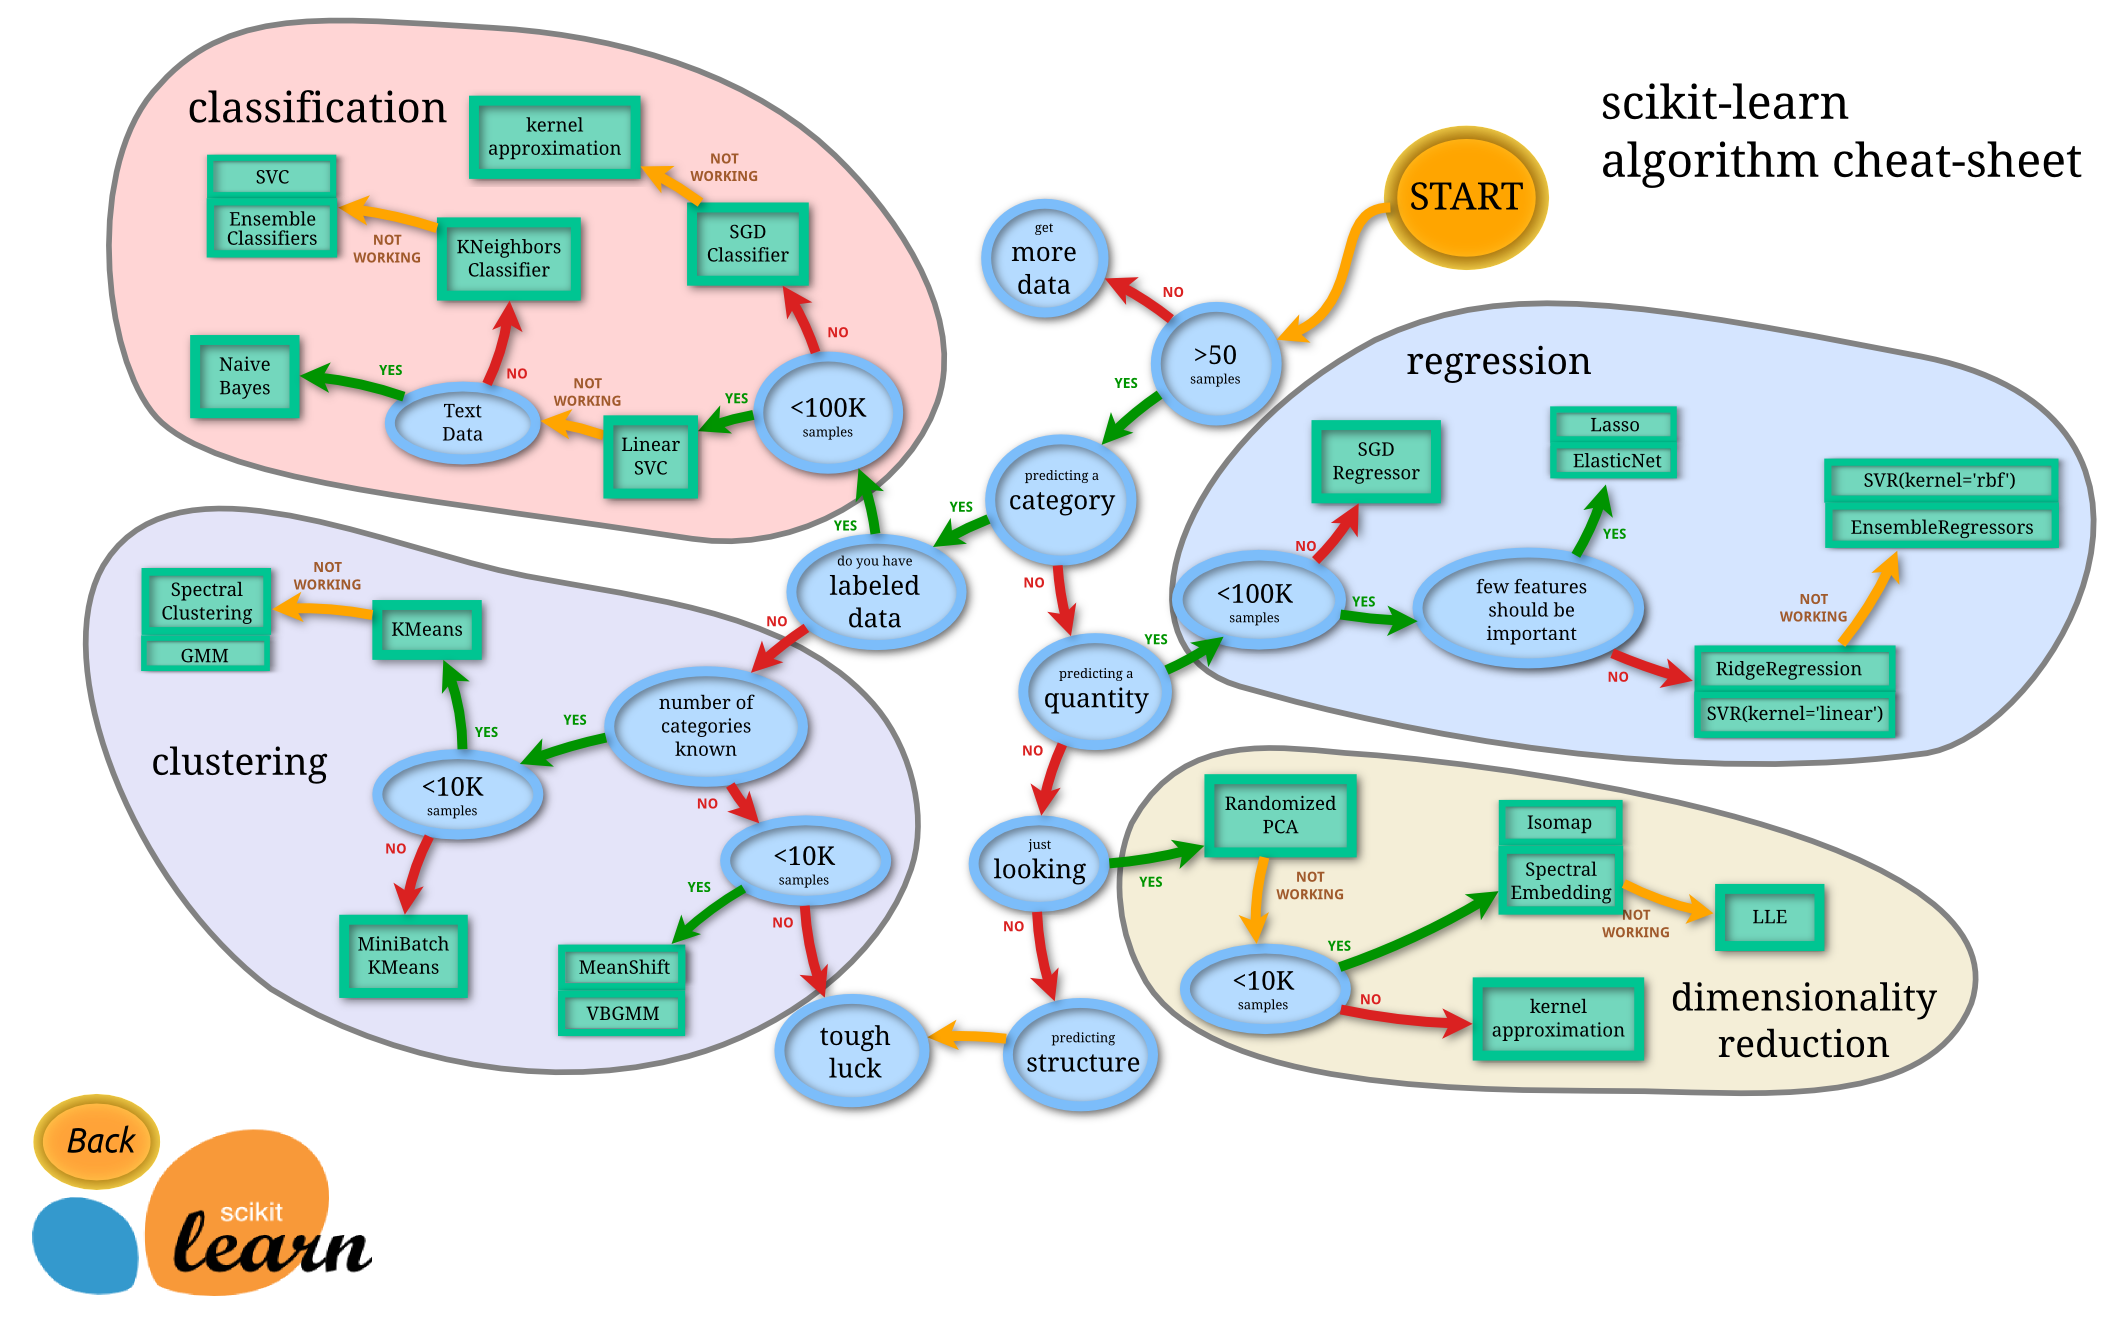
\includegraphics[width=.9\textwidth]{scikitlearn.png}

\end{frame}

%=============================================================================%
%=============================================================================%
\begin{frame}[fragile]
\frametitle{Scikit-learn}

\begin{lstlisting}[style=python]
from sklearn import datasets

# Load popular iris data set
iris = datasets.load_iris()
xTrain = iris.data # petal/sepal width/length
yTrain = iris.target 
\end{lstlisting}

% import matplotlib.pyplot as plt
% # Keep only petal width and sepal length
% xTrain = iris.data[:, [3, 0]] # petal width and sepal length

% # Plot data
% plt.scatter(xTrain[:, 0], xTrain[:, 1], c="black")
% plt.xlabel("Petal width")
% plt.ylabel("Sepal length")
\vspace{-0.5cm}
\centering
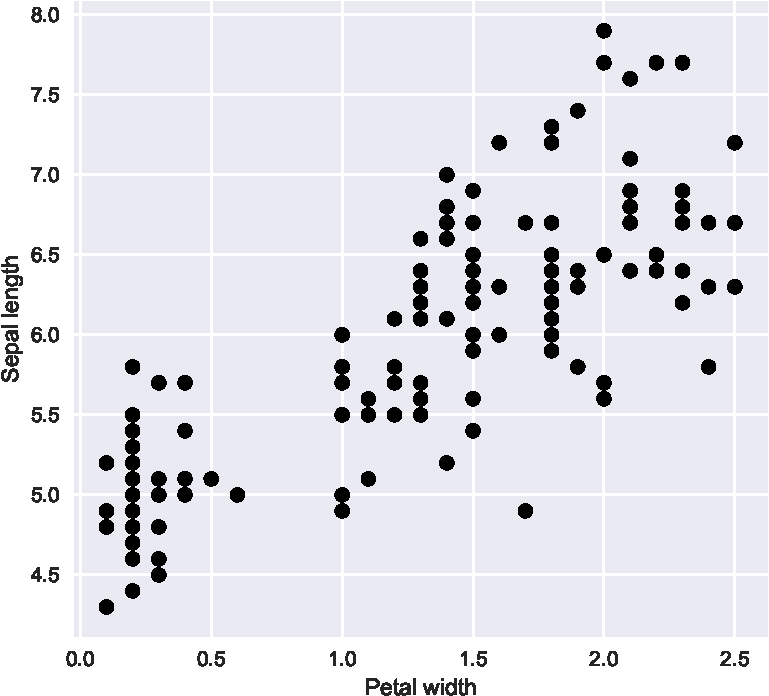
\includegraphics[width=.45\textwidth]{kmeans1.pdf}

\end{frame}

%=============================================================================%
%=============================================================================%
\begin{frame}[fragile]
\frametitle{Scikit-learn: k-means clustering}

\begin{lstlisting}[style=python]
from sklearn.cluster import KMeans

# Set up k-means clustering model
model = KMeans(n_clusters=3)

# Fit model with supplied data (unsupervised)
model.fit(xTrain)
\end{lstlisting}
% # Extract labels
% labels = model.labels_

% # Map labels to colour
% col = []

% for label in labels:
%     if label == 0:
%         col.append("blue")
%     elif label == 1:
%         col.append("red")
%     elif label == 2:
%         col.append("green")
%     else:
%         col.append("grey")
            

% # Plot data and colour by cluster
% plt.scatter(xTrain[:, 0], xTrain[:, 1], c=col)
% plt.xlabel("Petal width")
% plt.ylabel("Sepal length"))

\vspace{-0.5cm}
\centering
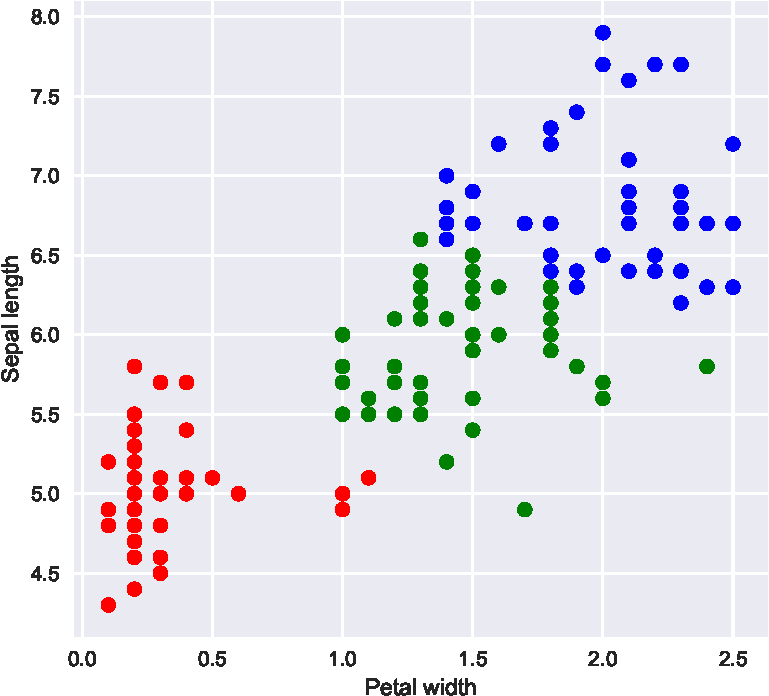
\includegraphics[width=.45\textwidth]{kmeans2.pdf}

\end{frame}

%=============================================================================%
%=============================================================================%
\begin{frame}[fragile]
\frametitle{Scikit-learn: Random forests}

\begin{lstlisting}[style=python]
from sklearn.ensemble import RandomForestClassifier

# Set up Random Forest model
model = RandomForestClassifier(n_estimators=500, oob_score=True)

# Fit model with supplied data (supervised)
model.fit(xTrain, yTrain)
\end{lstlisting}

% yTrain = []
% for i in iris.target:
%     if i==0:
%         yTrain.append("Setosa")
%     elif i==1:
%         yTrain.append("Versicolor")
%     else:
%         yTrain.append("Virginica")

% # Compute confusion matrix (actual vs predicted label)
% predLabel = [model.classes_[i] for i in list(model.oob_decision_function_.argmax(axis=1))]
% confusionMatrix = confusion_matrix(yTrain, predLabel)
% print(confusionMatrix)

\centering
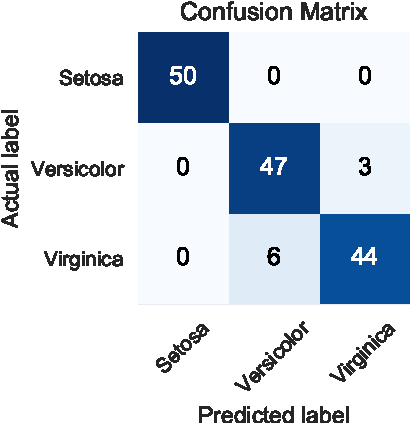
\includegraphics[width=0.35\textwidth]{confusion_matrix.pdf}

\end{frame}

%=============================================================================%
%=============================================================================%
\begin{frame}[fragile]
\frametitle{Networkx}

\href{https://networkx.github.io/}{\texttt{networkx}} is a package 
for the creation, manipulation, and study of the structure, dynamics, and functions of complex networks

\vfill

\begin{columns}
\column{0.65\textwidth}
\begin{lstlisting}[style=python]
import networkx as nx

# Creating a new empty Graph object
g = nx.Graph()

# Adding nodes
g.add_nodes_from(["Tom", "Zoe", 
                  "JJ", "Anna", "Peter"])

# Adding an edge
g.add_edge("JJ", "Zoe")
g.add_edge("JJ", "Anna")
g.add_edge("JJ", "Tom")
g.add_edge("Peter", "Zoe")
g.add_edge("Tom", "Anna")

# Draw network
nx.draw(g, node_size=1500, 
        with_labels=True)
\end{lstlisting}

\column{0.35\textwidth}
\centering
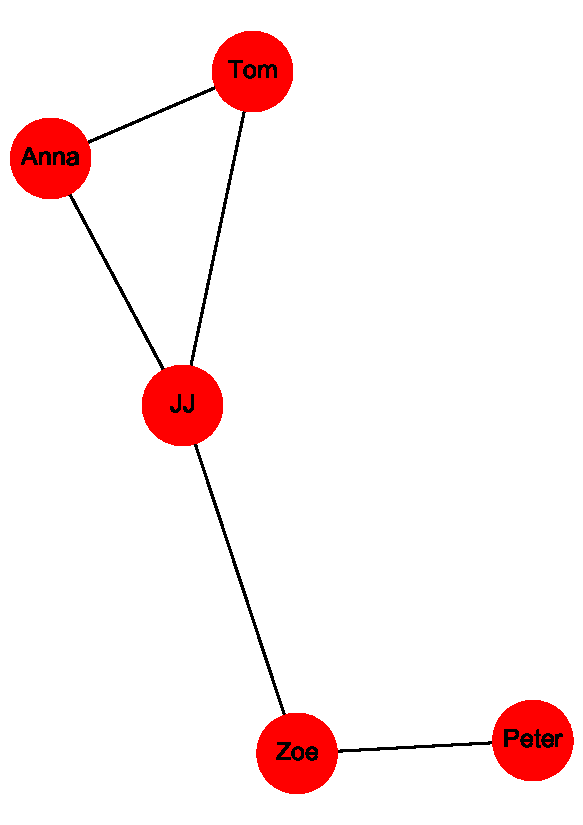
\includegraphics[width=\textwidth]{netx.pdf}
\end{columns}

\end{frame}

%=============================================================================%
%=============================================================================%
\begin{frame}[fragile]
\frametitle{ArcGIS}

\href{https://developers.arcgis.com/python/}{\texttt{arcgis}} is a package 
for GIS visualisation and analysis, spatial data management and GIS system
administration tasks

\vspace{0.2cm}

\begin{lstlisting}[style=python]
from arcgis.gis import GIS

# Create a GIS object (anonymous user)
gis = GIS()

# Get map of Cornwall
myMap = gis.map("Cornwall, UK")
myMap
\end{lstlisting}

\vspace{-0.5cm}

\centering
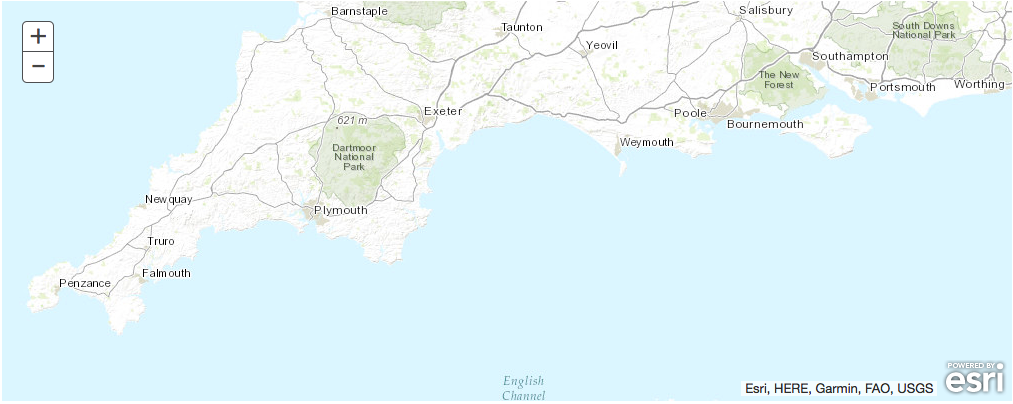
\includegraphics[width=.7\textwidth]{arcgis.png}

\end{frame}

%=============================================================================%
%=============================================================================%
\begin{frame}[fragile]
\frametitle{MyGene}

\href{http://docs.mygene.info/projects/mygene-py/en/latest/}{\texttt{mygene}} provides 
web services to query/retrieve gene annotation data from \href{http://mygene.info/}{MyGene.info}

\vspace{0.2cm}

\begin{lstlisting}[style=python]
import mygene

# Instantiate MyGeneInfo class
mg = mygene.MyGeneInfo() 

# Query for the name and EnsemblID of genes Ifng and Ccl3
mg.querymany(qterms=["Ifng", "Ccl3"], scopes="symbol", 
             fields=["name", "ensembl"], species="human") 
\end{lstlisting}

\vspace{-0.8cm}
{\fontsize{8}{8}\selectfont
\begin{verbatim}
[{'_id': '3458',
  '_score': 98.66912,
  'ensembl': {'gene': 'ENSG00000111537',
   'protein': 'ENSP00000229135',
   'transcript': 'ENST00000229135',
   'translation': [{'protein': 'ENSP00000229135', 'rna': 'ENST00000229135'}]},
  'name': 'interferon gamma',
  'query': 'Ifng'},
....
....
....
\end{verbatim}}

\end{frame}

%=============================================================================%
%=============================================================================%
\begin{frame}[fragile]
\frametitle{Tweepy}

\href{http://www.tweepy.org/}{\texttt{tweepy}} provides
access to Twitter for posting/reading tweets
\\[0.5em]
How about analysing tweets from
\href{https://keithselover.wordpress.com/2016/08/31/a-look-at-trump-and-clintons-tweets-using-tweepy-part-2-term-frequency/}{Mr President}?

\vspace{0.3cm}

\centering
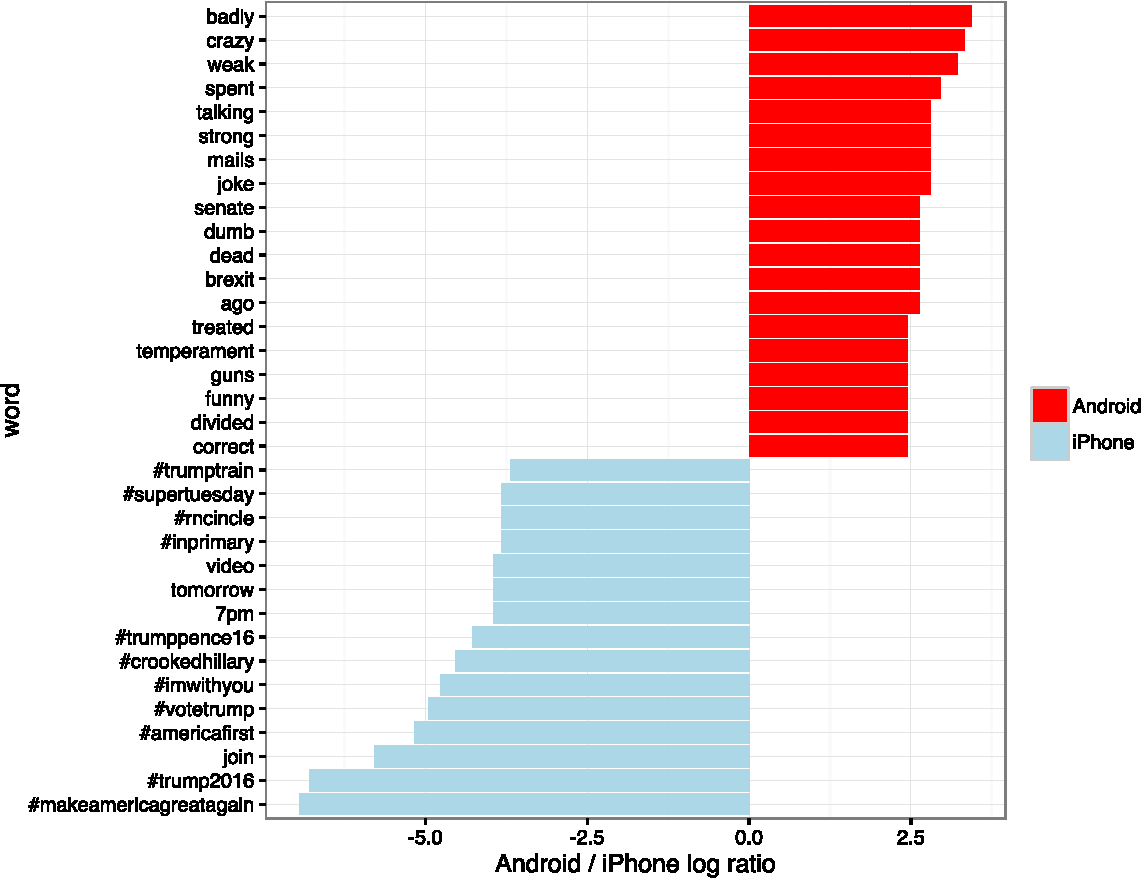
\includegraphics[width=.65\textwidth]{tweepy.pdf}

\scriptsize
Image taken from \href{http://varianceexplained.org/r/trump-tweets/}{here} (analysis done in R) 
\normalsize

\end{frame}

%=============================================================================%
%=============================================================================%
% End of Document
%=============================================================================%
%=============================================================================%
\end{document}
